% \chapter*{Abstract}
\addcontentsline{toc}{chapter}{Abstract} 

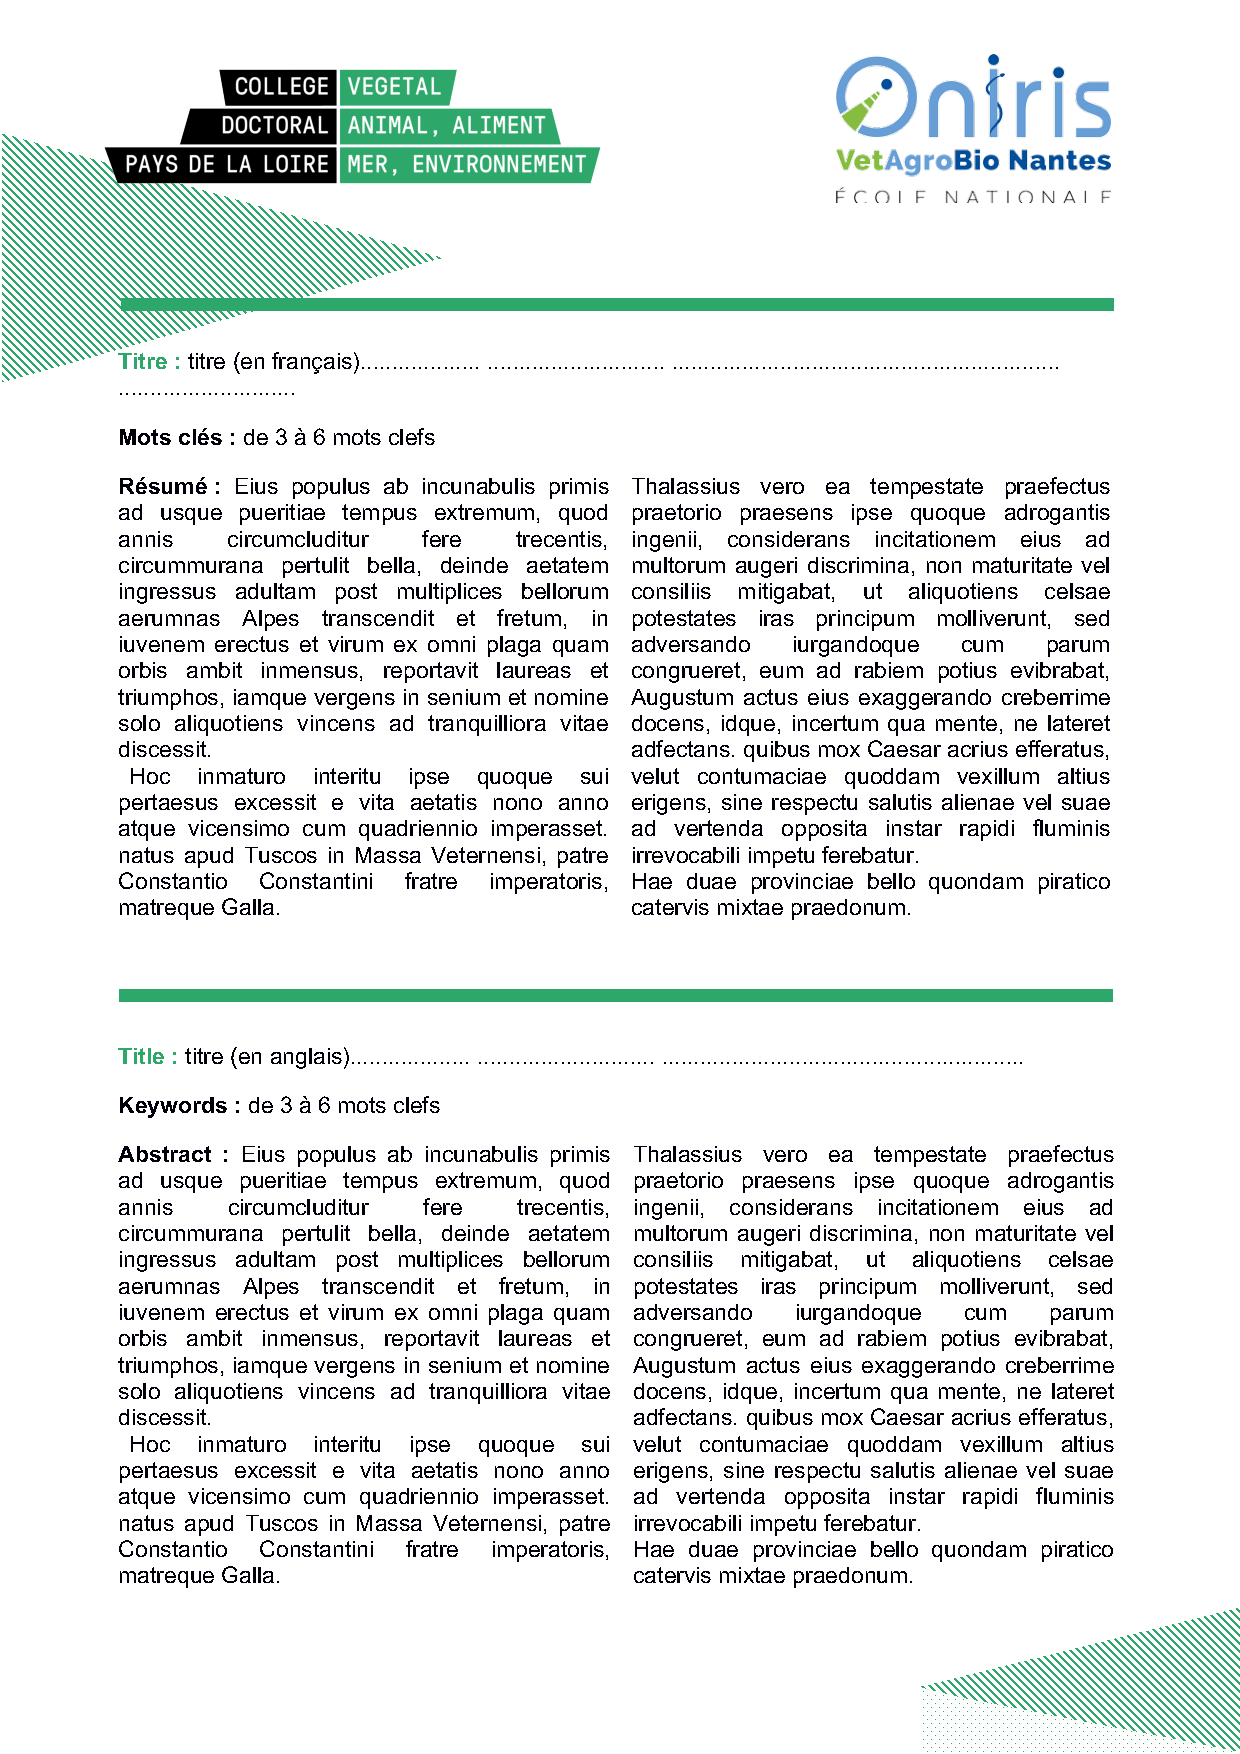
\includepdf[pages=1]{figures/ED_requirements/Abstract.pdf}

	
% \newpage
% \thispagestyle{empty}


% \mbox{}
% \newpage

% Bovine Respiratory Disease (BRD) is a common and complex infectious illness in cattle that causes significant health and economic losses. Sensor technologies in modern livestock farming can monitor animal health in real time, but current sensor-based alerts often lack specificity and generate too many false alarms. This thesis proposes a novel hybrid approach that combines deep learning and mechanistic epidemiological modeling to transform raw sensor observations into reliable insights for disease detection and control. Deep neural networks provide quick diagnoses from sensor data (such as ultrasound images), while mechanistic models use these diagnostics to simulate the spread and outcomes of disease over longer periods. Applied to BRD using data from nine French cattle farms, this integrated method improves early detection of outbreaks and filters out uncertain cases to avoid false interventions. The hybrid model achieved high accuracy in detecting sick animals and significantly reduced false positive alerts. It also informed smarter antibiotic use, cutting unnecessary treatments by around 44% and slightly improving economic outcomes (~1% increase in profit). These findings demonstrate the potential of merging AI-driven diagnostics with epidemiological models to produce accurate and interpretable predictions, better supporting farmers and veterinarians in managing livestock diseases. Keywords: Bovine Respiratory Disease, sensor-based diagnostics, deep learning, epidemiological modeling, precision livestock farming, decision support